% Chapter: Results and Discussion
% ACTIVE (2026-08-03): chapter uncommented and populated with exemplar prose
% built around the verified simulation results. Every prose paragraph is
% wrapped in EXEMPLAR markers for the user to rewrite in their own words.

\section{Solver Verification}
\label{sec:res_verification}

% --- EXEMPLAR PARAGRAPH (rewrite in your own words) ---
Before any transfer function was trusted, the solver of \refSec{sec:meth_solver} was verified by the method of manufactured solutions and by grid and timestep convergence studies.
In the manufactured-solution test, an analytic source term is added to the kinetics so that a known field solves the equations exactly, and the discrete error is measured as the grid and the time step are refined.
Three configurations were tested: the Barkley kinetics with isotropic diffusion, the Barkley kinetics with a tilted anisotropic diffusion tensor, and the Oregonator kinetics at candidate A.
\reffig{fig:res_mms} shows the measured error norms against grid spacing and time step.
The observed spatial convergence orders at the finest refinement interval are $2.09$, $2.09$, and $1.99$ for the three cases, against a design order of $2$ for the central-difference diffusion operator.
The observed temporal orders are approximately $1.0$ across all cases and error norms, matching the first-order operator splitting of \refSec{sec:meth_discretisation}.
The tilted-tensor case converges at the same rate as the isotropic case, which validates the divergence-form tensor discretisation that the anisotropy experiment of \refSec{sec:res_anisotropy} depends on.
% --- END EXEMPLAR ---

\begin{figure}[htbp]
\centering
\IfFileExists{../Analysis/figures/rd_mms.png}{%
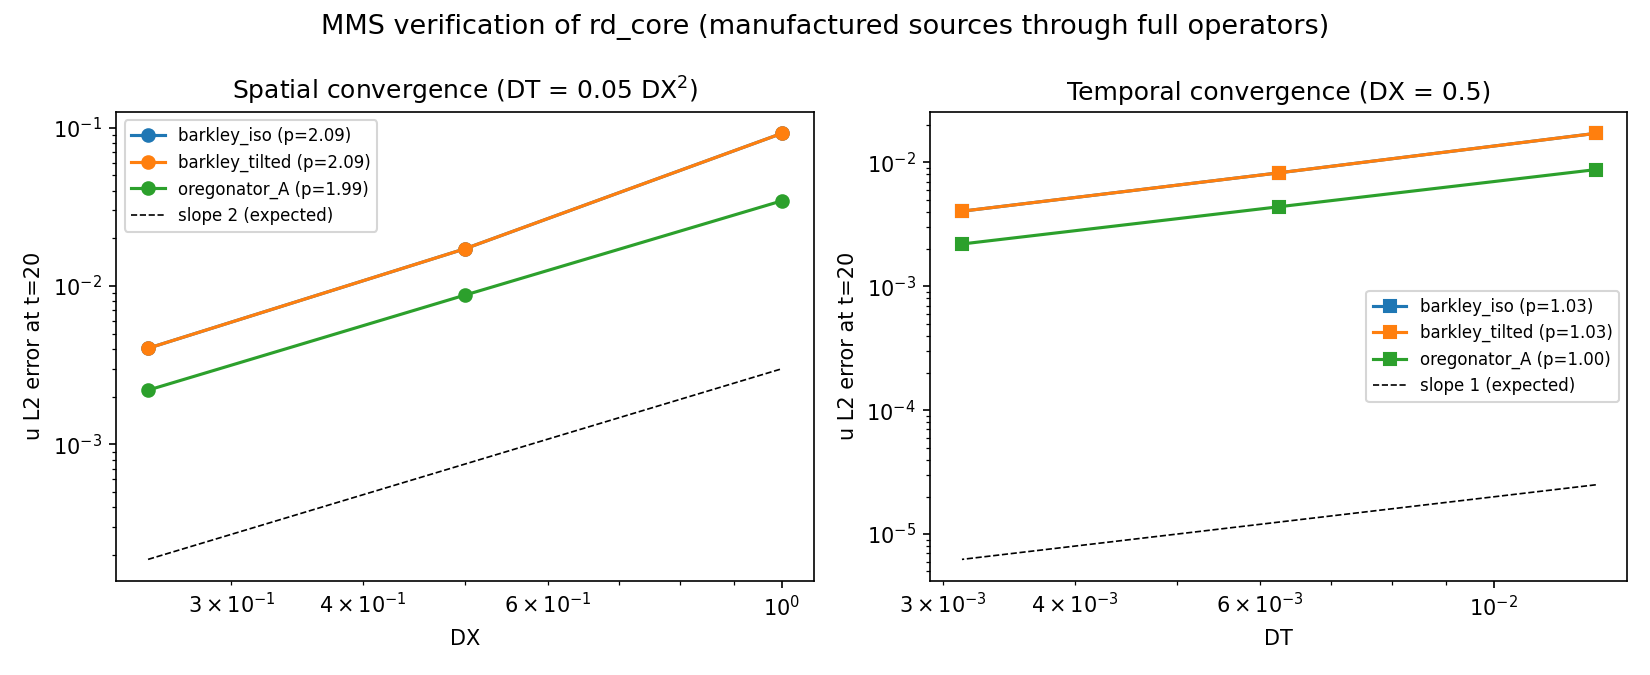
\includegraphics[width=0.9\textwidth]{../Analysis/figures/rd_mms.png}}{%
[figure pending]}
\caption{Method of manufactured solutions: measured error norms against grid spacing (spatial convergence) and time step (temporal convergence) for three configurations, Barkley isotropic, Barkley with a tilted anisotropic tensor, and Oregonator candidate A. Observed spatial orders are $2.09$, $2.09$, and $1.99$ against a design order of $2$; observed temporal orders are approximately $1.0$ against a design order of $1$. The tilted-tensor case converges like the isotropic case.}
\label{fig:res_mms}
\end{figure}

% --- EXEMPLAR PARAGRAPH (rewrite in your own words) ---
Convergence of the physical quantity of interest, the plane-pulse speed, is summarised in \reftab{tab:res_convergence} and \reffig{fig:res_verification}.
The Barkley speed rises monotonically from $4.151$ cells per time unit at $\Delta x = 1$ to $4.603$ at $\Delta x = 0.25$.
A Richardson extrapolation of the three refinement levels gives a continuum asymptote of approximately $4.82$ cells per time unit, so the working resolution underestimates the Barkley speed by about $14\%$.
The observed order of the sequence is only about $0.8$: the refinement is still pre-asymptotic, because the pulse front is only two to three cells thick at these resolutions and is not yet smooth enough on the grid for asymptotic convergence.
The Oregonator candidate-A speeds, $6.224$, $6.048$, and $6.049$ cells per time unit across the same refinement, lie within a $2.8\%$ band, so the Oregonator measurements are close to grid-converged at the working resolution.
Timestep refinement changes measured speeds and timings by at most $1.5\%$ for both kinetics at the working step $\Delta t = 0.05$.
A joint $(\Delta x, \Delta t)$ refinement map shows the error to be space-dominated and approximately separable: at fixed $\Delta x$, temporal refinement contributes less than $0.7\%$ further change.
% --- END EXEMPLAR ---

\begin{table}[htbp]
\centering
\caption{Grid convergence of the plane-pulse speed (cells per time unit) at $\Delta t = 0.05$. The Barkley sequence is pre-asymptotic (observed order $\approx 0.8$); a Richardson extrapolation gives a continuum asymptote of $\approx 4.82$, a deficit of $\approx 14\%$ at the working resolution $\Delta x = 1$. The Oregonator candidate-A speeds lie within a $2.8\%$ band.}
\label{tab:res_convergence}
\small
\begin{tabular}{@{}ccc@{}}
\toprule
\textbf{$\Delta x$ (cells)} & \textbf{Barkley speed} & \textbf{Oregonator A speed} \\
\midrule
1.00 & 4.151 & 6.224 \\
0.50 & 4.439 & 6.048 \\
0.25 & 4.603 & 6.049 \\
\midrule
Richardson asymptote & $\approx 4.82$ & n/a \\
\bottomrule
\end{tabular}
\end{table}

\begin{figure}[htbp]
\centering
\IfFileExists{../Analysis/figures/rd_verification.png}{%
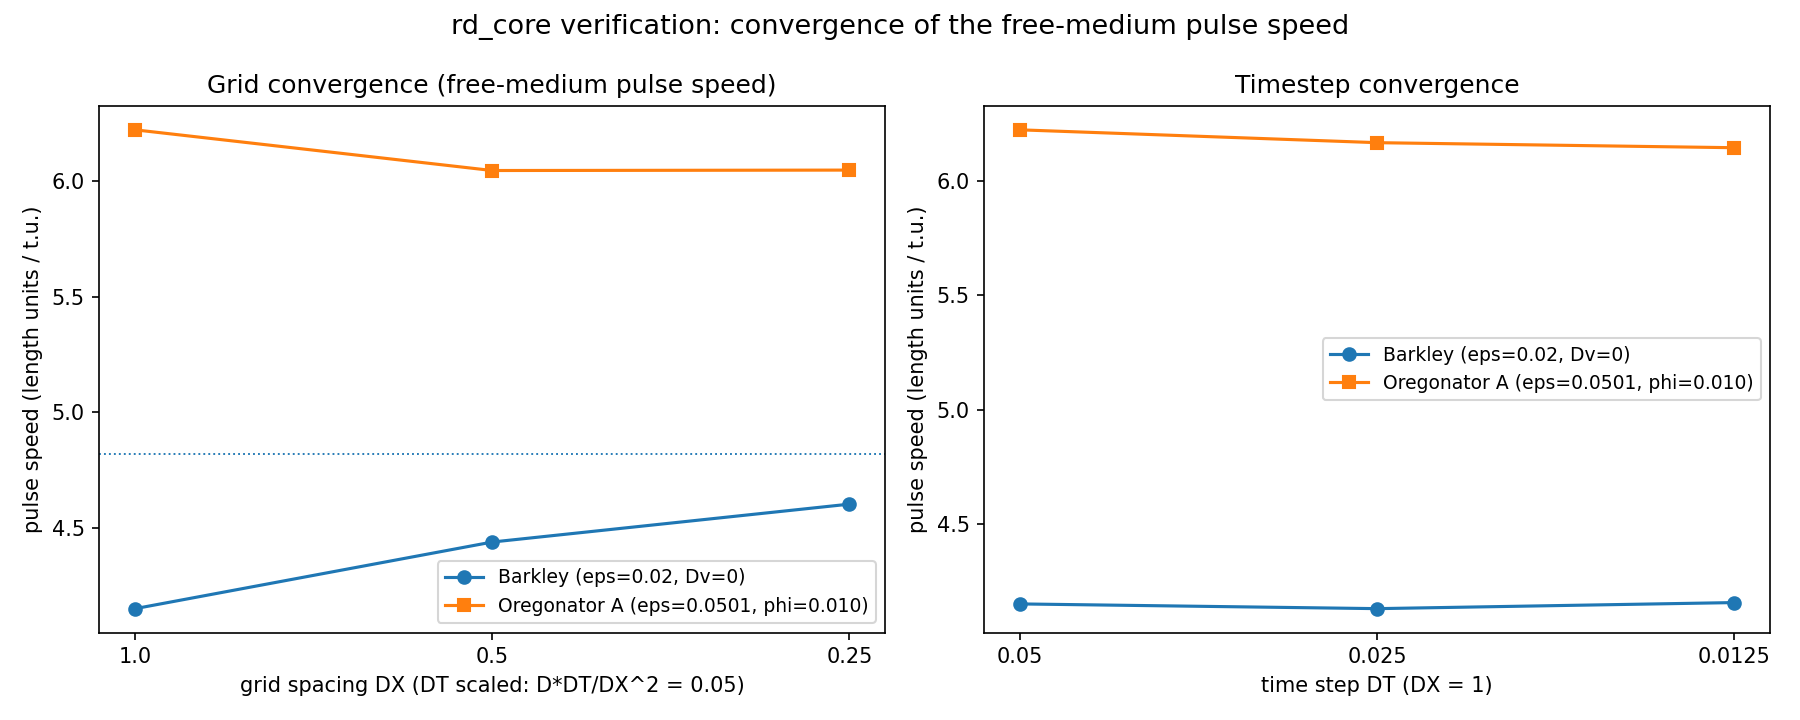
\includegraphics[width=0.9\textwidth]{../Analysis/figures/rd_verification.png}}{%
[figure pending]}
\caption{Solver verification summary: plane-pulse speed against grid spacing for both kinetics, timestep convergence at the working grid, and the joint $(\Delta x, \Delta t)$ error map. The Barkley refinement sequence is monotonic and pre-asymptotic toward the Richardson asymptote $\approx 4.82$ cells per time unit; the Oregonator sequence is flat within a $2.8\%$ band. The error is space-dominated and separable, with less than $0.7\%$ temporal contribution at fixed $\Delta x$.}
\label{fig:res_verification}
\end{figure}

% --- EXEMPLAR PARAGRAPH (rewrite in your own words) ---
Every runtime invariant monitored in the simulations underlying this chapter was clean: the NaN/Inf tripwire never fired, and the step-size guard recorded zero trips outside the fast upstroke it was designed for.
All results reported below were produced by this verified solver.
% --- END EXEMPLAR ---

\section{Channel Pulse Transfer}
\label{sec:res_channel}

% --- EXEMPLAR PARAGRAPH (rewrite in your own words) ---
The first component characterised is the wire.
In the free medium, a plane pulse travels at $4.151$ cells per time unit with the Barkley kinetics and at $6.223$ cells per time unit with the Oregonator at candidate A.
\reffig{fig:res_channel} shows the measured transfer of a single pulse along a straight walled channel as the channel width $W$ is swept down to a single cell.
The result is exact and somewhat surprising: the speed measured in the channel is bit-identical to the free-medium speed at every width tested, down to $W = 1$ cell, and the pulse transmits with undiminished amplitude.
No geometric wave block was observed at any width; the eikonal critical width below which confinement would extinguish the pulse is sub-grid for this medium.
% --- END EXEMPLAR ---

% --- EXEMPLAR PARAGRAPH (rewrite in your own words) ---
The physics of this result is clean.
A pulse travelling in a straight channel is a planar front, and a planar front has zero curvature, so the eikonal curvature correction to its speed vanishes \cite{keener1991eikonal}.
The no-flux walls impose a zero normal derivative on the activator field, which a planar front already satisfies identically; the walls therefore change nothing, and propagation in the channel is exactly equivalent to propagation on a one-dimensional cable.
The width-induced block documented in ring and cable studies \cite{courtemanche1993instabilities} requires the front to acquire curvature, which a straight uniform channel never forces on it.
As a device characteristic the result cuts both ways: a straight channel is a near-perfect wire whose speed and amplitude are set by the kinetics alone, but the width of a straight guide offers no computing leverage.
Structure that computes must come from junctions, curvature, or the property fields, not from confinement alone.
% --- END EXEMPLAR ---

\begin{figure}[htbp]
\centering
\IfFileExists{../Analysis/figures/rd_transfer_channel_final2.png}{%
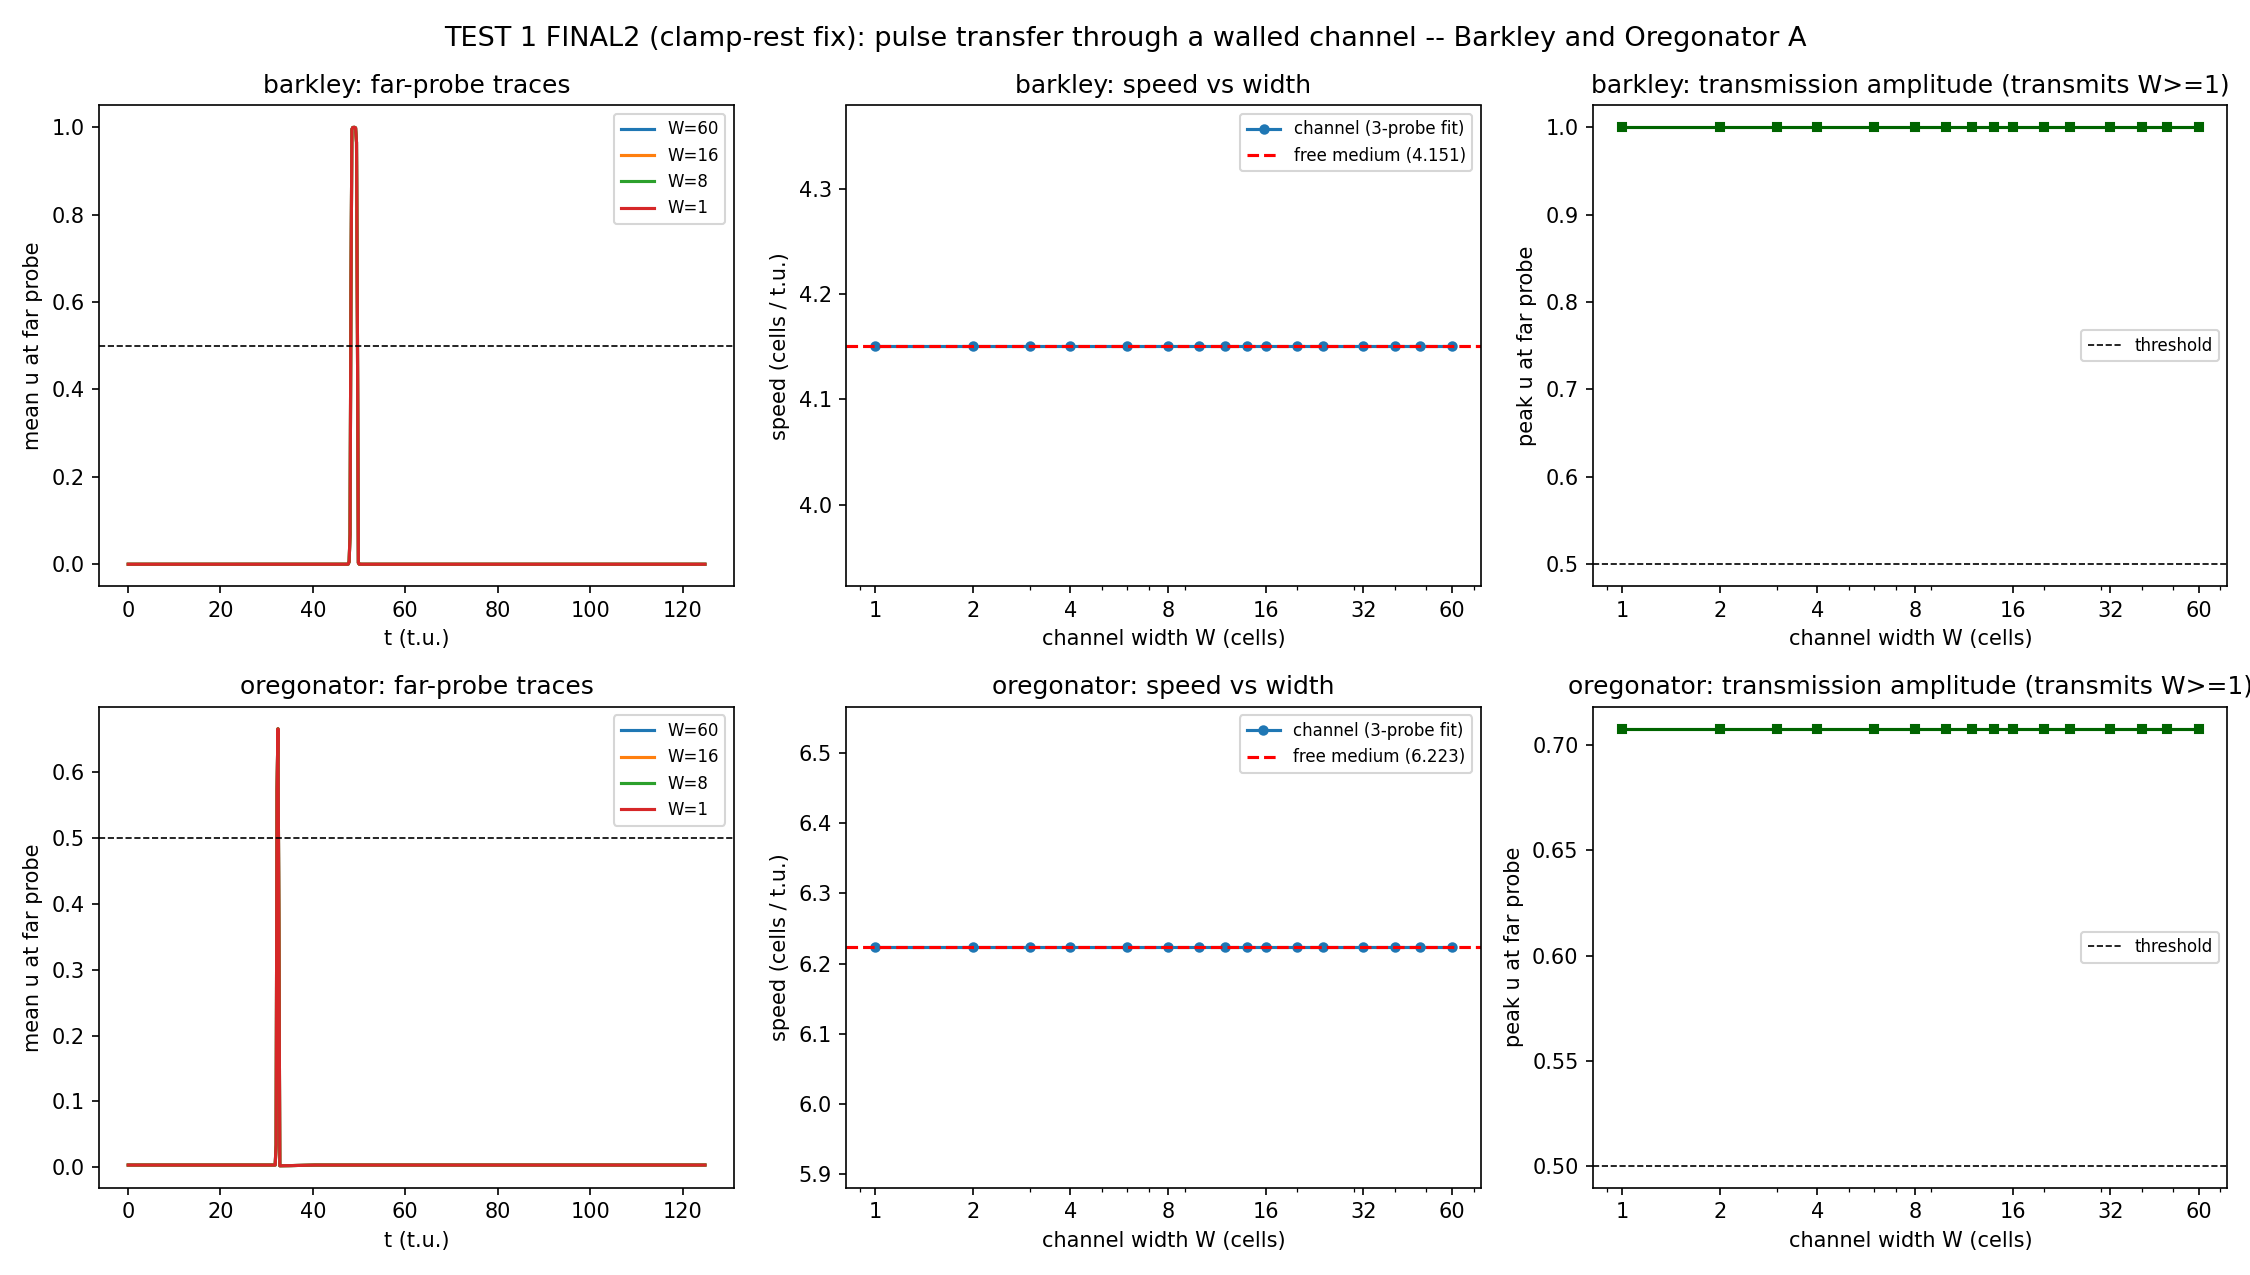
\includegraphics[width=0.9\textwidth]{../Analysis/figures/rd_transfer_channel_final2.png}}{%
[figure pending]}
\caption{Channel pulse transfer. Measured pulse speed in straight walled channels of width $W$ down to one cell, for both kinetics. The channel speed is bit-identical to the free-medium speed ($4.151$ cells per time unit Barkley, $6.223$ Oregonator A) at every width: a planar front between no-flux walls is exactly equivalent to a one-dimensional cable, and no geometric wave block occurs.}
\label{fig:res_channel}
\end{figure}

\section{Frequency Response}
\label{sec:res_frequency}

% --- EXEMPLAR PARAGRAPH (rewrite in your own words) ---
The second experiment measures the substrate's bandwidth, which is set by refractoriness.
The two-pulse measurement locates the absolute refractory period directly: $2.80$ time units for the Barkley kinetics, $3.10$ time units for the Oregonator at candidate A, and $2.70$ time units at candidate B.
Sustained pulse trains then give the transmission curves of \reffig{fig:res_frequency_barkley} and \reffig{fig:res_frequency_oregonator}.
At low input frequency the output frequency follows the input one-to-one: the curve has unit slope and every pulse transmits.
The maximum 1:1 following rate is $0.263$ per time unit for the Barkley kinetics and $0.282$ per time unit for the Oregonator at candidate A, rising to $0.323$ per time unit at candidate B.
Above this rate the curve leaves the unit slope and develops a staircase of dropped pulses, in which the medium locks to rational transmission ratios as more and more input pulses arrive inside the refractory wake of their predecessors.
% --- END EXEMPLAR ---

% --- EXEMPLAR PARAGRAPH (rewrite in your own words) ---
Two features of the measurement deserve note.
First, the maximum 1:1 following rate lies below the naive estimate given by the inverse of the absolute refractory period: in a sustained train each pulse propagates into the only partially recovered wake of the previous one, travels more slowly, and so extends the effective refractory interval.
This kind of rate-dependent transfer is familiar from measured transfer functions of excitable cables \cite{delange2009transfer}.
Second, the computational reading is direct: refractoriness is the substrate's clock limit.
Any signal encoding must space pulses by more than the refractory time, and any cascade of devices must operate below the maximum following rate.
The same property is also a native filter: the channel low-passes pulse trains for free, the same mechanism the junction literature exploits for frequency selection \cite{gorecka2003tshaped}.
% --- END EXEMPLAR ---

\begin{figure}[htbp]
\centering
\IfFileExists{../Analysis/figures/rd_transfer_frequency_final2_barkley.png}{%
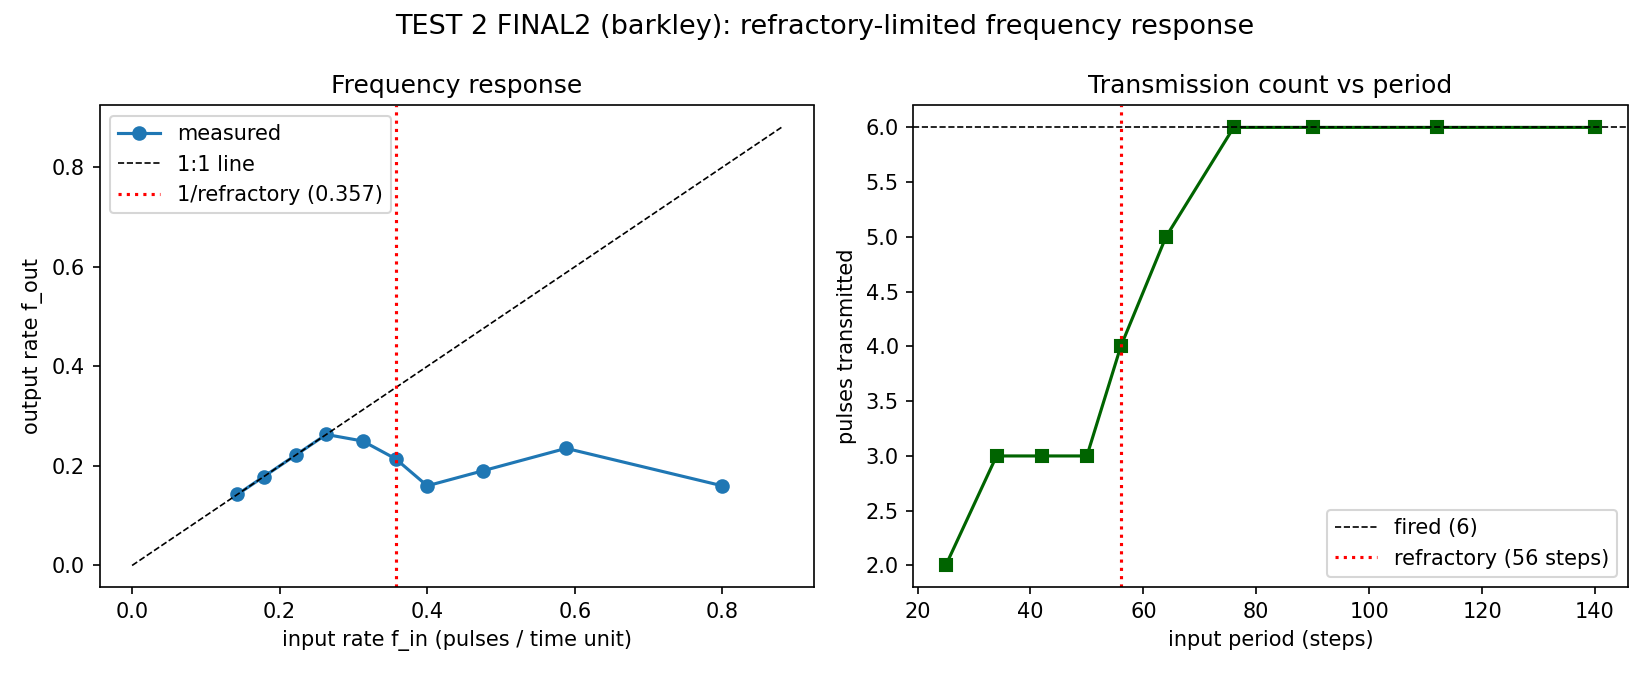
\includegraphics[width=0.85\textwidth]{../Analysis/figures/rd_transfer_frequency_final2_barkley.png}}{%
[figure pending]}
\caption{Frequency response of a channel with the Barkley kinetics. Two-pulse measurement locating the absolute refractory period at $2.80$ time units, and output against input frequency for sustained pulse trains. The 1:1 following region holds up to $0.263$ per time unit; above it the transmission curve forms a staircase of dropped pulses.}
\label{fig:res_frequency_barkley}
\end{figure}

\begin{figure}[htbp]
\centering
\IfFileExists{../Analysis/figures/rd_transfer_frequency_final2_oregonator.png}{%
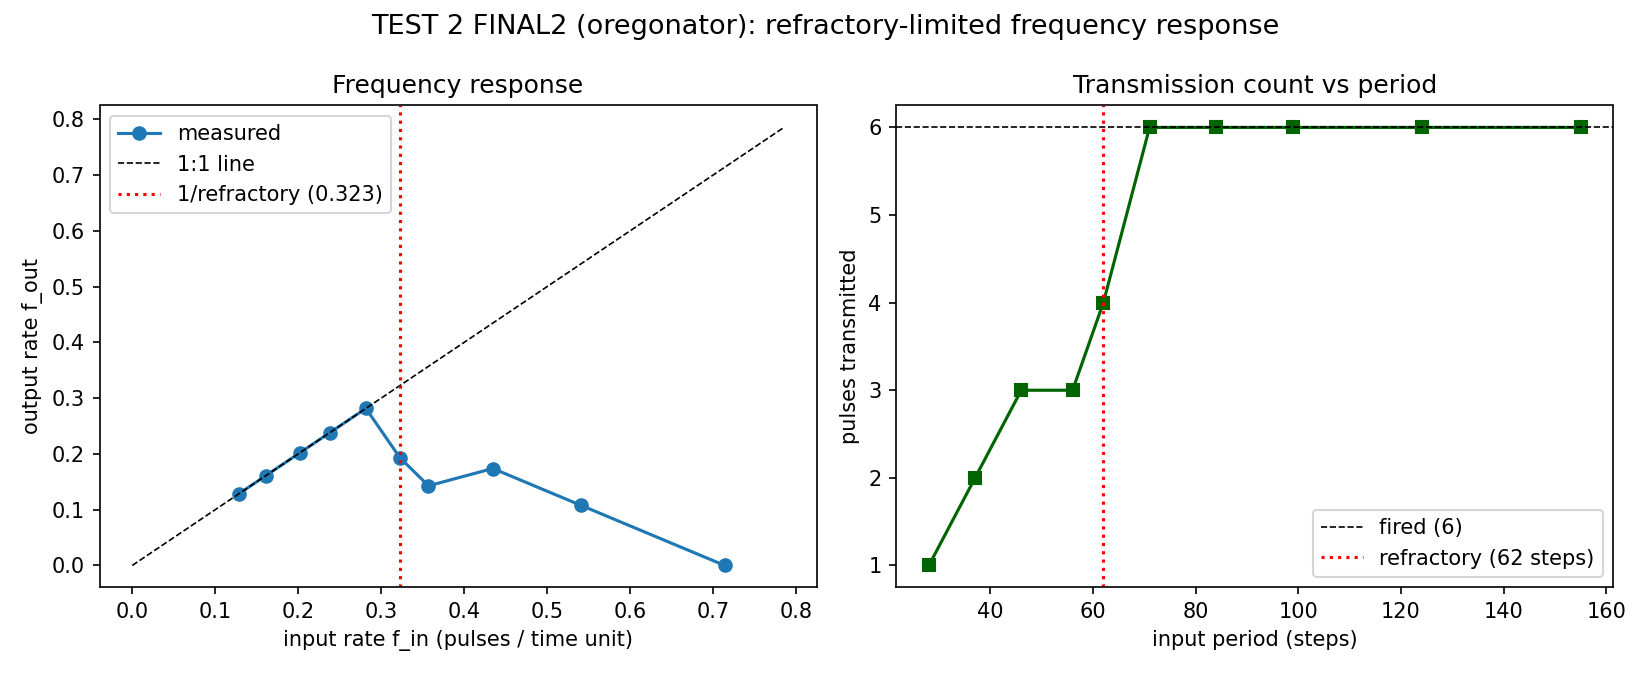
\includegraphics[width=0.85\textwidth]{../Analysis/figures/rd_transfer_frequency_final2_oregonator.png}}{%
[figure pending]}
\caption{Frequency response of a channel with the Oregonator kinetics. The absolute refractory period is $3.10$ time units at candidate A ($2.70$ at candidate B); the maximum 1:1 following rate is $0.282$ per time unit at candidate A ($0.323$ at candidate B). The staircase structure above the following limit reproduces the Barkley measurement.}
\label{fig:res_frequency_oregonator}
\end{figure}

\section{Two-Input Collision Logic}
\label{sec:res_logic}

% --- EXEMPLAR PARAGRAPH (rewrite in your own words) ---
The third experiment measures the substrate's native logic at a T-junction, with one input channel per arm and a probe on the output branch.
The first finding is negative and important: read naively over the whole record, the junction computes OR, whatever it was designed to do.
A lone pulse arriving on either arm diffracts into every connected branch, so the output probe fires whenever either input fires.
The complementary construction, annihilation XOR, in which coincident pulses cancel while lone pulses pass, is not realised by the passive junction alone, because the diffracted copies of a lone pulse reach the output probe unconditionally.
This is consistent with the collision-computing literature, where working gates rely on precisely timed inputs and purpose-built geometry rather than on an unadorned junction \cite{toth1995logic, steinbock1996chemical, adamatzky2002xor}.
% --- END EXEMPLAR ---

% --- EXEMPLAR PARAGRAPH (rewrite in your own words) ---
With the windowed readout of \refSec{sec:meth_protocol}, the same junction implements a genuine two-input gate.
The probe record is read only within a window aligned to the expected arrival of a lone pulse from the designated through-arm, input A.
If input B fires within the coincidence interval, its pulse collides with the A pulse at the junction, the two fronts annihilate, and the window reads silent.
\reftab{tab:res_truth} gives the measured truth table: the windowed device computes the inhibition gate A AND (NOT B), with B acting as a veto on A.
\reffig{fig:res_logic} shows the probe records underlying the table, and \reffig{fig:res_logic_snapshots} shows the corresponding wave fields.
% --- END EXEMPLAR ---

\begin{table}[htbp]
\centering
\caption{Measured truth table at the T-junction output probe, Barkley kinetics. Read over the whole record the junction computes OR, because lone pulses diffract into all branches. Read within the calibrated time window it computes the inhibition gate A AND (NOT B): input B vetoes input A through collision annihilation.}
\label{tab:res_truth}
\small
\begin{tabular}{@{}cccc@{}}
\toprule
\textbf{Input A} & \textbf{Input B} & \textbf{Naive readout (OR)} & \textbf{Windowed readout (A AND NOT B)} \\
\midrule
0 & 0 & 0 & 0 \\
0 & 1 & 1 & 0 \\
1 & 0 & 1 & 1 \\
1 & 1 & 1 & 0 \\
\bottomrule
\end{tabular}
\end{table}

% --- EXEMPLAR PARAGRAPH (rewrite in your own words) ---
Three figures of merit quantify the gate.
The separation ratio, the weakest true output against the strongest false one, is approximately $1000\times$ for the Barkley kinetics, a value capped by the probe noise floor rather than by the physics, and $232\times$ and $276\times$ for the Oregonator at candidates A and B.
The inhibition window, the range of relative input timings within which the trailing pulse is still annihilated, spans $2.0$ to $4.0$ time units.
The window also yields the design rule for scaling such gates: the difference in input-arm lengths must be engineered against the distance a pulse covers within the window, $c$ times $2.0$ to $4.0$ cells, since an asymmetry beyond that budget lets the veto pulse arrive too late to collide.
The device should therefore be understood as timing-gated rather than as pure combinational logic: its truth table holds only for inputs synchronised within the measured window, and the readout window is part of the device.
% --- END EXEMPLAR ---

\begin{figure}[htbp]
\centering
\IfFileExists{../Analysis/figures/rd_transfer_logic_final2_barkley.png}{%
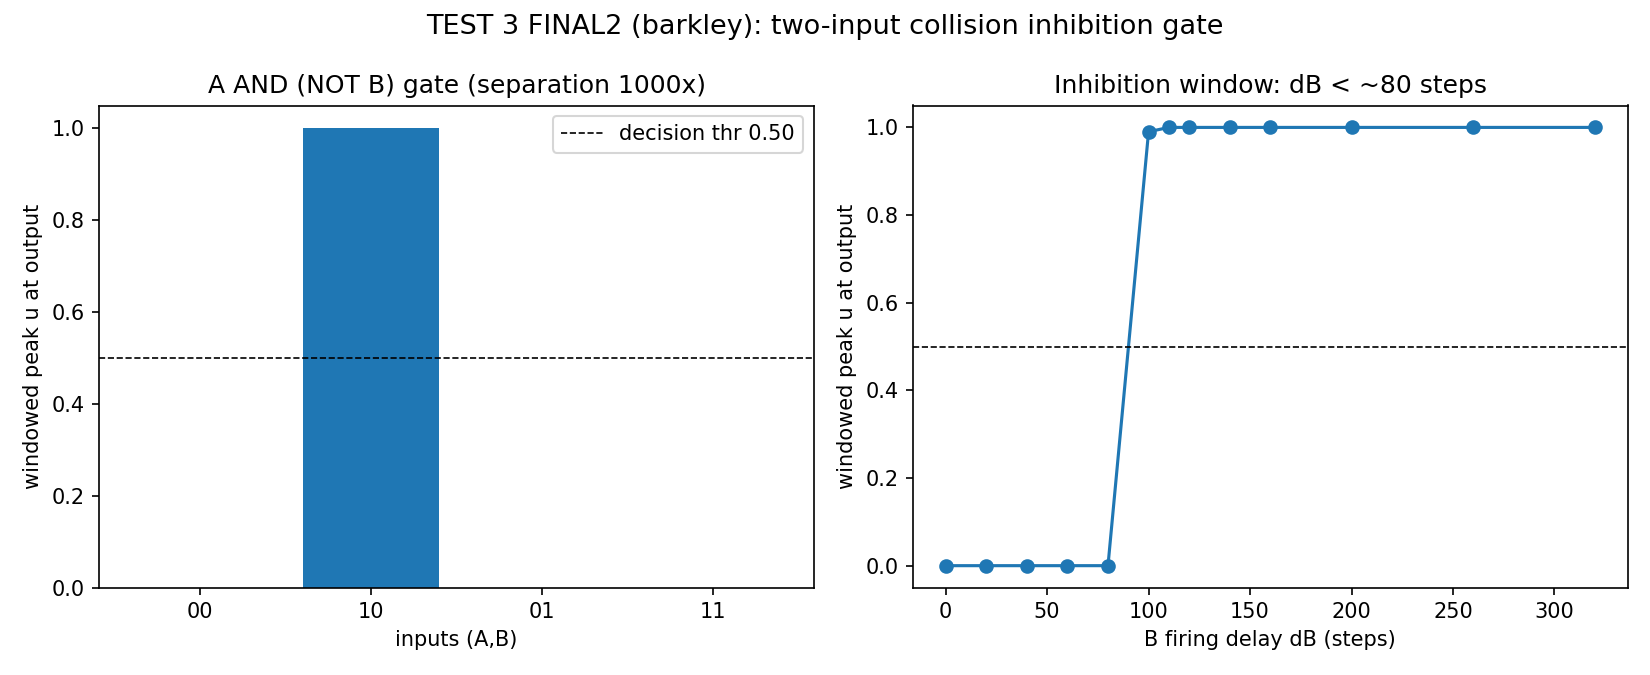
\includegraphics[width=0.9\textwidth]{../Analysis/figures/rd_transfer_logic_final2_barkley.png}}{%
[figure pending]}
\caption{Two-input collision logic at a T-junction, Barkley kinetics. Probe records for the four input combinations, with the calibrated readout window marked. A lone A pulse transmits; a B pulse within the coincidence interval annihilates it, giving the inhibition gate A AND (NOT B) with a separation ratio of approximately $1000\times$ (floor-capped).}
\label{fig:res_logic}
\end{figure}

\begin{figure}[htbp]
\centering
\IfFileExists{../Analysis/figures/rd_transfer_logic_final2_snapshots_barkley.png}{%
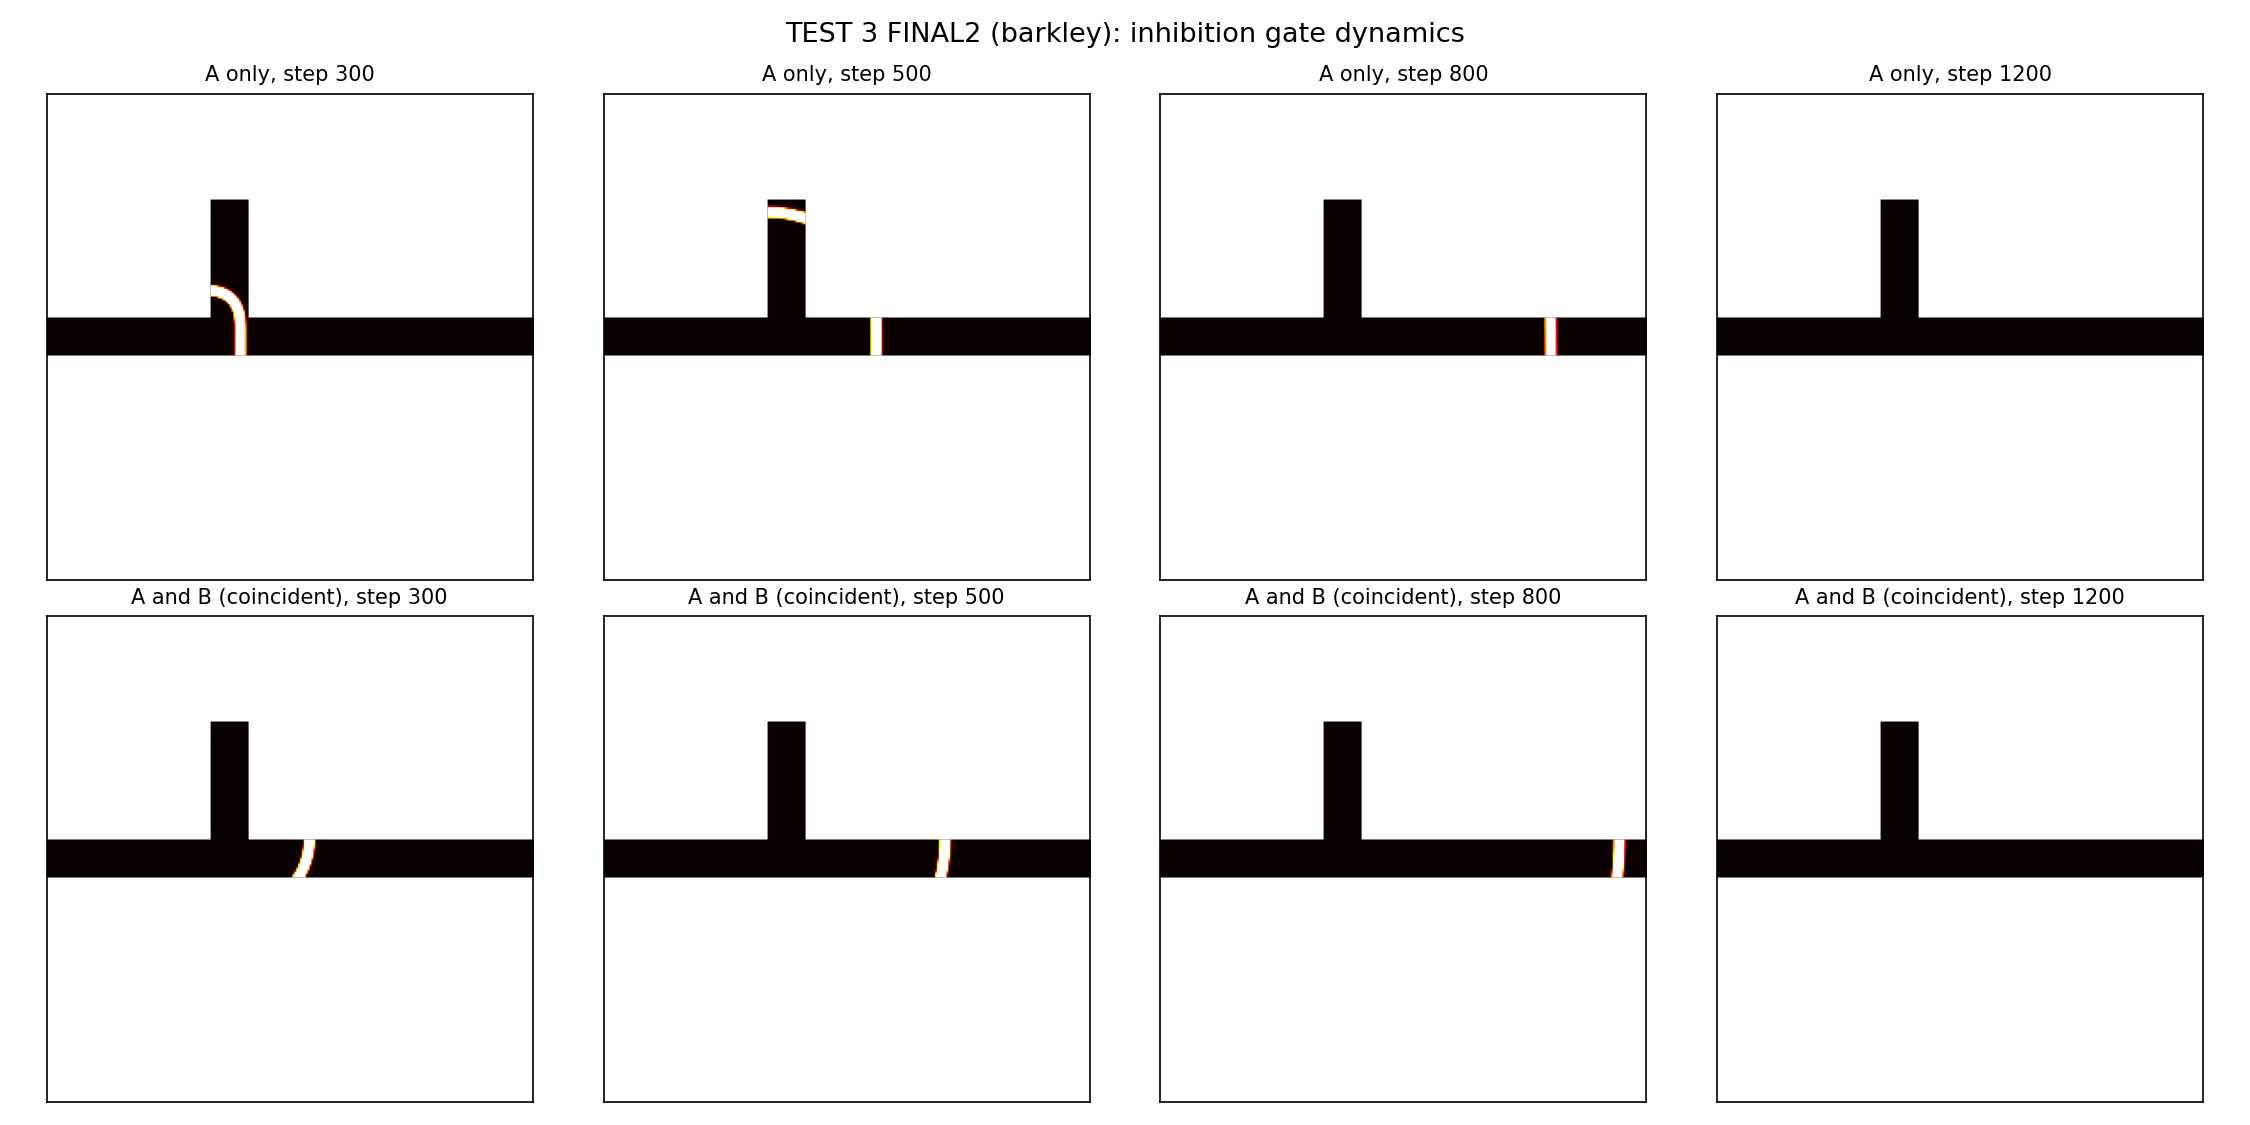
\includegraphics[width=0.9\textwidth]{../Analysis/figures/rd_transfer_logic_final2_snapshots_barkley.png}}{%
[figure pending]}
\caption{Wave-field snapshots of the collision gate, Barkley kinetics. Lone pulses diffract through the junction into all branches (the OR background); coincident pulses collide at the junction and annihilate, leaving the output branch silent within the readout window.}
\label{fig:res_logic_snapshots}
\end{figure}

\section{Anisotropic Substrate}
\label{sec:res_anisotropy}

% --- EXEMPLAR PARAGRAPH (rewrite in your own words) ---
The fourth experiment characterises the anisotropic parameterisation of \refSec{sec:meth_anisotropy}.
In a uniform tensor field with anisotropy ratio $r = D_{\parallel}/D_{\perp}$, eikonal theory predicts an elliptical pulse front whose axis ratio, and whose speed ratio between the fast and slow directions, scales as $\sqrt{r}$ \cite{keener1991eikonal}.
The measured front geometry follows this law closely, as \reffig{fig:res_aniso} shows.
The isotropic control $r = 1$ reproduces the circular front exactly.
At $r = 2$ the deviation from the $\sqrt{r}$ prediction is $4.6\%$ for the Barkley kinetics and $0.24\%$ for the Oregonator; at $r = 4$ it is $9.6\%$ and $0.34\%$ respectively.
At $r = 8$ the Barkley deviation reaches $10.2\%$, which remains within the $\approx 14\%$ spatial error bar established for that kinetics in \refSec{sec:res_verification}.
The full directional speed profile $c(\theta)$, probed along rays at several orientations to the fibre direction, matches the elliptic theory to within $1.2\%$.
The tensor discretisation is therefore quantitatively trustworthy, and the residual Barkley deviations are accounted for by the known, openly stated grid error rather than by any failure of the anisotropic formulation.
% --- END EXEMPLAR ---

% --- EXEMPLAR PARAGRAPH (rewrite in your own words) ---
The device-relevant measurement embeds a patch of anisotropic medium in the isotropic substrate and records the delay a pulse accumulates crossing it.
As the fibre direction of the patch is rotated from parallel ($0$ degrees) to perpendicular ($90$ degrees) to the incident propagation direction, the transmission delay grows monotonically from $644$ to $836$ time steps.
The response is smooth, monotone, and continuous in the fibre angle: the patch acts as a continuously tunable delay element, and two patches with different orientations route pulses along paths of different effective length without ever blocking them.
This is a routing capability that neither walls nor the light field provides, steering propagation direction in the interior of the medium rather than at its boundaries, in the spirit of patterned-excitability experiments \cite{steinbock1995anisotropy}.
% --- END EXEMPLAR ---

\begin{figure}[htbp]
\centering
\IfFileExists{../Analysis/figures/rd_transfer_aniso_final2.png}{%
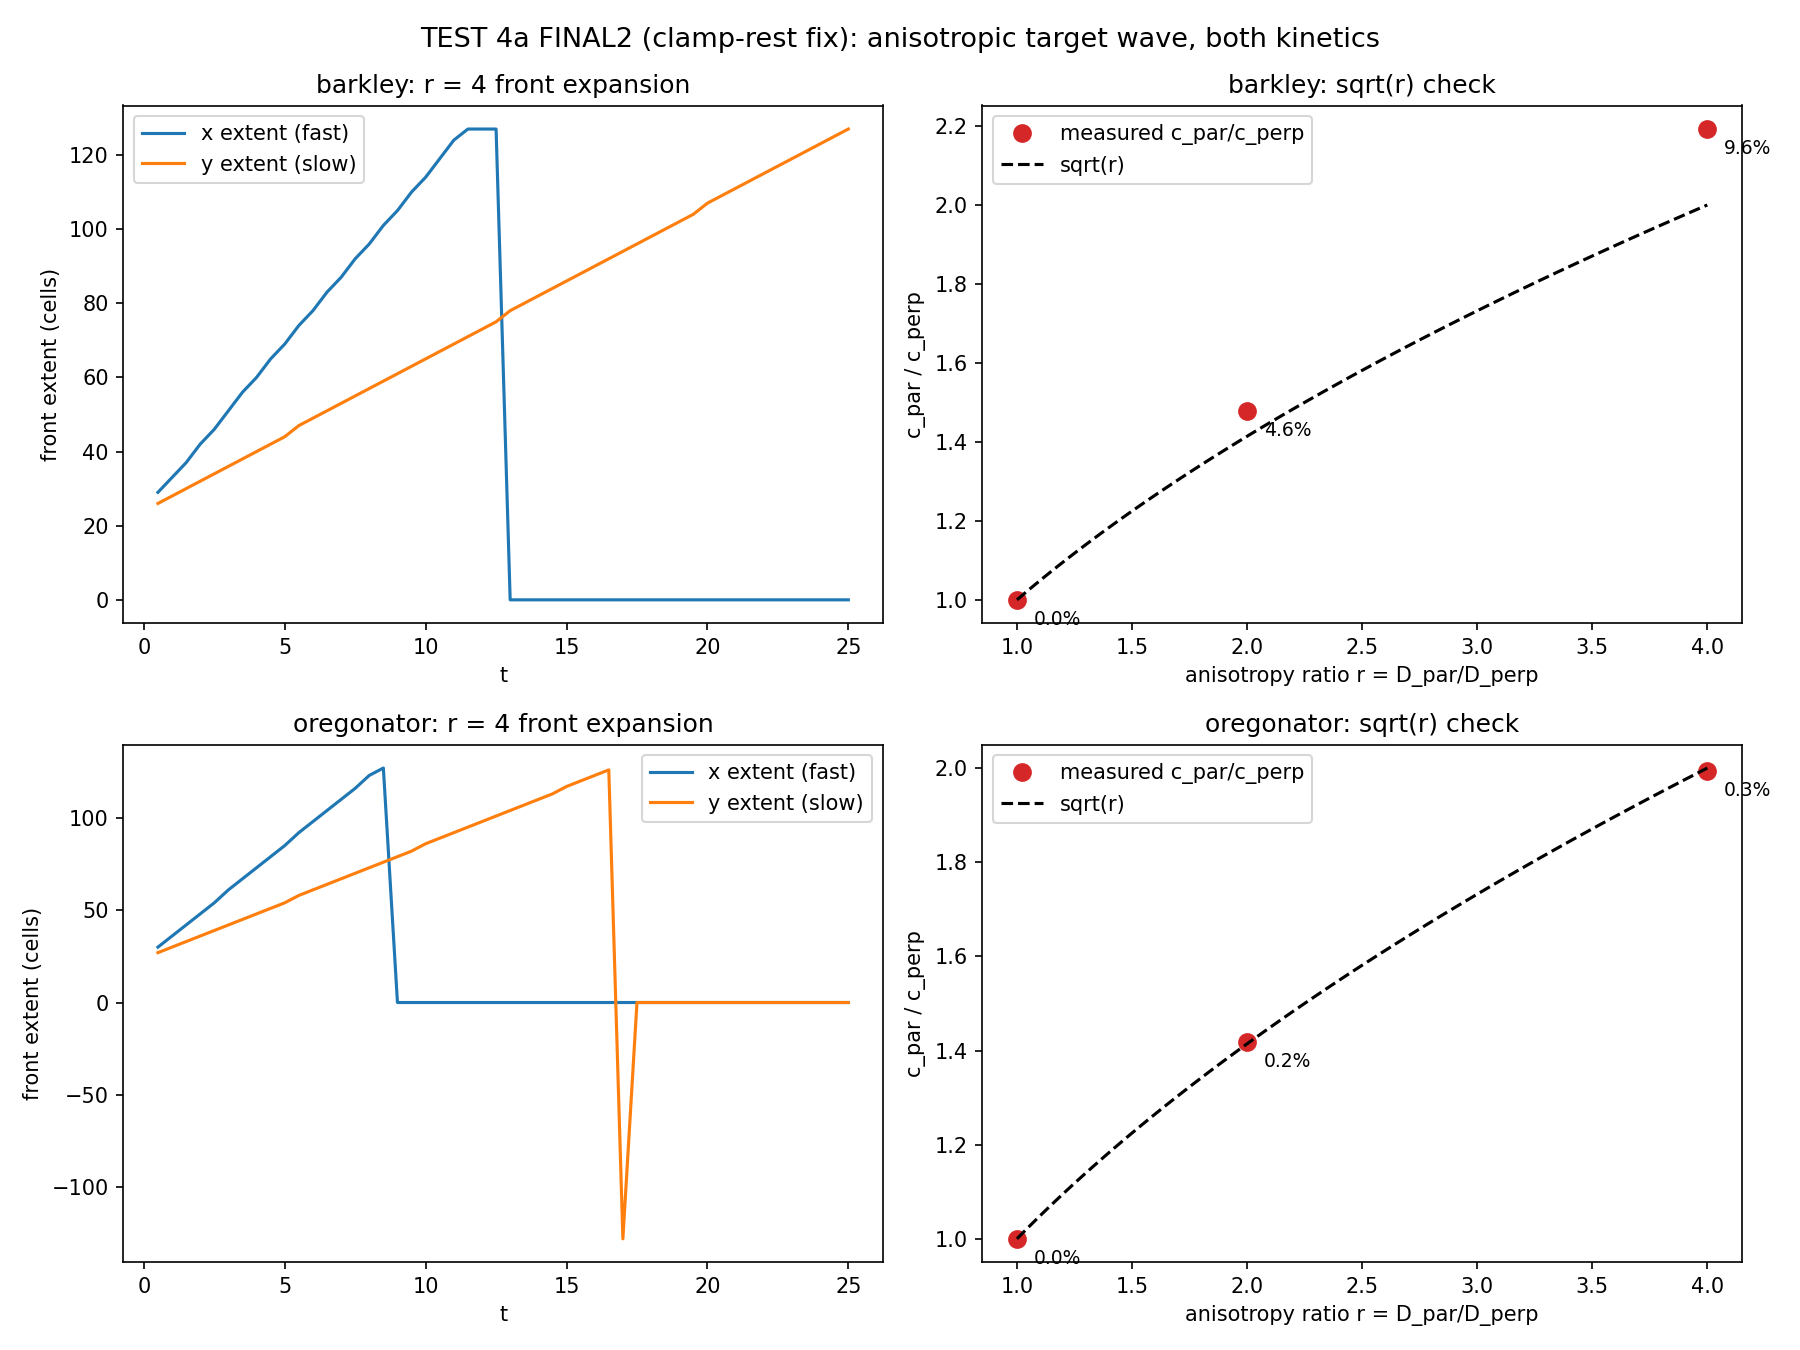
\includegraphics[width=0.9\textwidth]{../Analysis/figures/rd_transfer_aniso_final2.png}}{%
[figure pending]}
\caption{Anisotropic substrate. Elliptical pulse fronts in uniform tensor fields follow the $\sqrt{r}$ eikonal law (deviations $4.6$--$10.2\%$ Barkley, $\leq 0.34\%$ Oregonator, for $r = 2$ to $8$); the directional speed profile $c(\theta)$ matches theory to $1.2\%$; and the transmission delay across an embedded anisotropic patch grows monotonically from $644$ to $836$ time steps as the fibre angle rotates from $0$ to $90$ degrees.}
\label{fig:res_aniso}
\end{figure}

\section{Discussion}
\label{sec:res_discussion}

% --- EXEMPLAR PARAGRAPH (rewrite in your own words) ---
Read together, the four experiments constitute a component datasheet for the substrate.
It is a slow, parallel, threshold-logic medium.
Straight channels are near-ideal wires whose speed is set by the kinetics alone, though their width carries no computing leverage (\refSec{sec:res_channel}).
Refractoriness imposes a hard bandwidth ceiling, the medium's clock limit, and doubles as a native pulse-train filter (\refSec{sec:res_frequency}).
Junctions with windowed readout supply native inhibition logic, A AND (NOT B), from which arbitrary Boolean functions can in principle be composed, provided inputs are synchronised within the measured timing window (\refSec{sec:res_logic}).
Anisotropy adds continuous, non-blocking routing and delay control in the interior of the medium (\refSec{sec:res_anisotropy}).
Because every headline measurement was reproduced with two kinetics of different mathematical structure and different physical provenance, these transfer functions should be read as properties of excitable media generally, not as quirks of one model's parameterisation.
% --- END EXEMPLAR ---

% --- EXEMPLAR PARAGRAPH (rewrite in your own words) ---
In the physical-neural-network framing of \refSec{sec:lit_pnn}, the characterisation defines what training would buy.
The native transfer functions are fixed by the kinetics; the three substrate parameterisations of \refSec{sec:meth_parameterisation} reshape them.
Walls are the coarse, binary program: they place the ports, wires, and junctions, but the channel experiment shows they contribute no graded behaviour of their own.
The light field $\phi(x,y)$ is the graded and experimentally rewritable knob \cite{sakurai2002design}, and the measurements reported here expose exactly the levers a training loop would pull: regime stability, propagation speed, timing, and block.
The anisotropic tensor is a continuous steering field with a verified quantitative law.
Closing the loop from this characterisation to actual training over $\phi(x,y)$ and the geometry was out of scope for the present work; the limitations of the study and the route to trained substrates are taken up in \refChap{chap:conclusions}.
% --- END EXEMPLAR ---
